% ---------------------------------------------------------------------
% -------------- PREAMBLE ---------------------------------------------
% ---------------------------------------------------------------------

%\documentclass[12pt,a4paper,finnish,oneside]{article}
\documentclass[lnbip]{svmultln}

\usepackage[utf8]{inputenc}
\usepackage[english]{babel}

\usepackage{calc}      % käytetään laskurien (counter) yhteydessä (tiedot.tex)
\usepackage{natbib}
\usepackage{url}
\usepackage{listings}
\usepackage{hyphenat}

\usepackage{supertabular,array}
\usepackage{lipsum}
\usepackage{booktabs}
\usepackage{graphicx}


% Strikethrough
\usepackage[normalem]{ulem}

% Punctuation for references
\bibpunct{[}{]}{;}{n}{,}{,}

% correct bad hyphenation here
\hyphenation{op-tical net-works semi-conduc-tor}


\usepackage{multibib}
\newcites{gen}{References}
\usepackage{bibentry}


% ---------------------------------------------------------------------
% -------------- DOCUMENT ---------------------------------------------
% ---------------------------------------------------------------------

\begin{document}

\selectlanguage{english}

\mainmatter

\title{Large scale agile transformations: A literature review}

\titlerunning{Large scale agile transformations}

\author{Kim Dikert \and Maria Paasivaara \and Casper Lassenius}
\authorrunning{Kim Dikert et al.}   % abbreviated author list (for running head)

% list of authors for the TOC (use if author list has to be modified)
\tocauthor{Kim Dikert, Maria Paasivaara, Casper Lassenius}

\institute{Aalto University . . . Address . . .
\\ \email{email@xx},
\\ WWW home page: \texttt{http://www...} }

\maketitle


% ---------------------------------------------------------------------
% -------------- ABSTRACT AND TEXT ------------------------------------
% ---------------------------------------------------------------------

\begin{abstract}        % give a summary of your paper
The abstract should summarize the contents of the paper
using at least 70 and at most 150 words. It will be set in 9-point
font size and be inset 1.0 cm from the right and left margins.
There will be two blank lines before and after the Abstract.
%                         please supply keywords within your abstract
\keywords {agile, transformation, large scale}
\end{abstract}


% ---------------------------------------------------------------------
\section{Introduction}

As the competition in software industry is growing companies are constantly
looking to improve their effectiveness. Agile methods are claimed to increase
productivity and quality \citegen{Livermore2008}, which makes them attractive for
companies pursuing better performance. However, large organizations may have
problems introducing agile methods \citegen{Dyba2009}. As agile methods are
initially designed for small teams their application has proven to be
problematic in a larger scale \citegen{Boehm2005}.

It is typical for large companies to function according to traditional software
engineering models [Cite?!] (also why?). These models strive for consistent quality and performance
by rigorous planning and definition of process. This kind of approach is however
badly suited for software development, as projects typically encounter
situations that are too hard or impossible to foretell \citegen{Schwaber2002}.
The main problems in plan-driven development are the high cost of changes and
late feedback on quality \citegen{Petersen2010}. Long release cycles, cost of
resopnding to change and distance from customers undermine the  competitiveness
of companies. Agile methods are believed to bring remedy to these problems.

The goal of this research is to explore how and why large organizations adopt
agile methods. Studies on large scale agile transformations have been published,
but no extensive and summarizing research is available on the subject. In this
research we will give an overview of reported case studies on adopting agile
methods in large organizations. We will further discuss the motivations for
adopting agile methods, the characteristics of agile transformations, and
factors relating to success or challenge in the transformation process. Our
research is focused on the process of organizational change. We leave out topics
related to comparing the initial and transformed states of organisations, such
as measuring the performance of organizations before and after the
transformation.

This paper is organized as follows. The next section gives an overview of large
scale agile development. Section \ref{sec:method} presents the literature review
method used for conducting the research. The findings of the review are
discussed in section \ref{sec:results}, and section \ref{sec:conclusions}
discusses the findings and gives proposals for future research.


% ---------------------------------------------------------------------
\section{Background}
\label{sec:background}

Introducing agile methods in large organizations is more difficult than it is in
small organizations \citegen{Dyba2008}. The difficulty is partly related to size
bringing higher organizational inertia which slows down organizational change
\citegen{Livermore2008}. Agile methods are not founded on the use of individual
tools or practices, but rather on a holistic change in the way of thinking.
Adopting agile requires often change of the entire organizational culture
\citegen{Misra2010}.

One significant difference between small and large adoptions is that large
organizations have more dependencies between projects and teams. This increases
the need for formal documentation and thus reduces agility \citegen{Lindvall2004}.
In addition to inter-team coordination large organizations require development
teams to interact with other organizational units, which are often non-agile of
their nature. For instance, HR may demand individuals to have strictly specified
roles in projects \citegen{Boehm2005}, or a change control board may inhibit use of
continuous integration or refactoring \citegen{Lindvall2004}. All units affected by
the agile transformation need to be informed and heard, and the agile process
must be adjusted according to their needs \citegen{Lindvall2004, Cohn2003,
Boehm2005}.

Agile methods will also affect management and business related functions. A key
challenge is that management must move away from life cycle models and towards
iterative and feature centric models \citegen{Nerur2005}. The focus must be shifted
from a large scale scope to shorter term project planning \citegen{Misra2010}, as
agile methods emphasize that meaningful planning can only be done for the near
future \citegen{Cohn2003}. However, the lack of planning can be a concern as
business and customer relationships often build on long term roadmapping.
Enabling operation with shorter term planning requires educating stakeholders
and reviewing contracting practices \citegen{Boehm2005}.


% ---------------------------------------------------------------------
\section{Research method}
\label{sec:method}

% Research questions:
%
% What are the motivations for starting an organizational transformation?
%
% What kind of agile transformations have been reported?
%
% What were challenges and success factors in the transformation process?


The literature review was conducted as an application of Kitchenham's
method for systematic literature review (SLR) \citegen{Kitchenham2007}. The method
was applied to be performed by only one researcher, and to serve as a
preliminary work evaluating the feasibility of a more in-depth review. The
required effort was limited by selecting only the following subset of SLR steps:
identification of primary sources, data extraction and synthesis. Steps left out
were the development of a systematic review protocol, strict study quality
assessment, and reviews in the study selection process.

\subsection{Data sources and search strategy}

The searches for primary sources was conducted in two steps. First a preliminary
search was made to sample the existing literature. Then a systematic search was
done based on the preliminary search. The following databases were included in
the searches: IEEExplore\footnote{http://ieeexplore.ieee.org/},
ACM\footnote{http://dl.acm.org/}, Scopus\footnote{http://www.scopus.com/},
ProQuest\footnote{http://search.proquest.com/}.
Additionally the archive of International XP
Conference\footnote{http://link.springer.com/} was searched.

The search phrases used in the preliminary search were \textit{agile
transformation} and \textit{large scale agile}. For the systematic search three
facets and appropriate keywords were chosen, as presented in Table
\ref{table:searchterms}. To search the databases a query phrase was constructed
by joining the keywords of each facet by \texttt{OR} operators and the facets by
\texttt{AND} operators.

As the preliminary search omitted some of the keywords in Table
\ref{table:searchterms} it yielded a small number of additional matches. The
reason for variance in matches was that many articles had creative titles or the
abstracts and keywords were not informative enough. Because of this, the search
with more restrictive keywords was unable to capture all possible matches.
We are however confident that the search covered the majority of material
relating to agile transformations in large organizations. If a wider search
should be performed, our recommendation is to only regard the facets
\textit{agile methods} and \textit{organizational change}. This would lead to
significantly more matches in the first stage of selecting studies, but the
additional effort is necessary due to the limitations of a keyword search.

\begin{table}[h]
    \begin{tabular}{ l@{ \hskip 0.4cm } l }
        \toprule
        Facet                  & Keywords   \\ \midrule
        Agile methods          & agile, scrum, lean, xp \\ 
        Organizational change  & transformation, transition, change, migration \\
        Large organization     & enterprise, organization, (large \texttt{AND} scale) \\
        \bottomrule
    \end{tabular}
    \caption{Facets and related search terms used}
    \label{table:searchterms}
\end{table}

The selection process of the primary studies is summarized in Figure
\ref{fig:selection_process}. The database search yielded 1603 matches from which
100 sources were chosen by the title. 17 unmatched sources from the preliminary
search were also included. Finally, 31 sources were selected based on the
abstract to be included for data extraction. One source was not available, which
reduced the final number of primary studies to 30.

\begin{figure}[htb]
  \begin{center}
    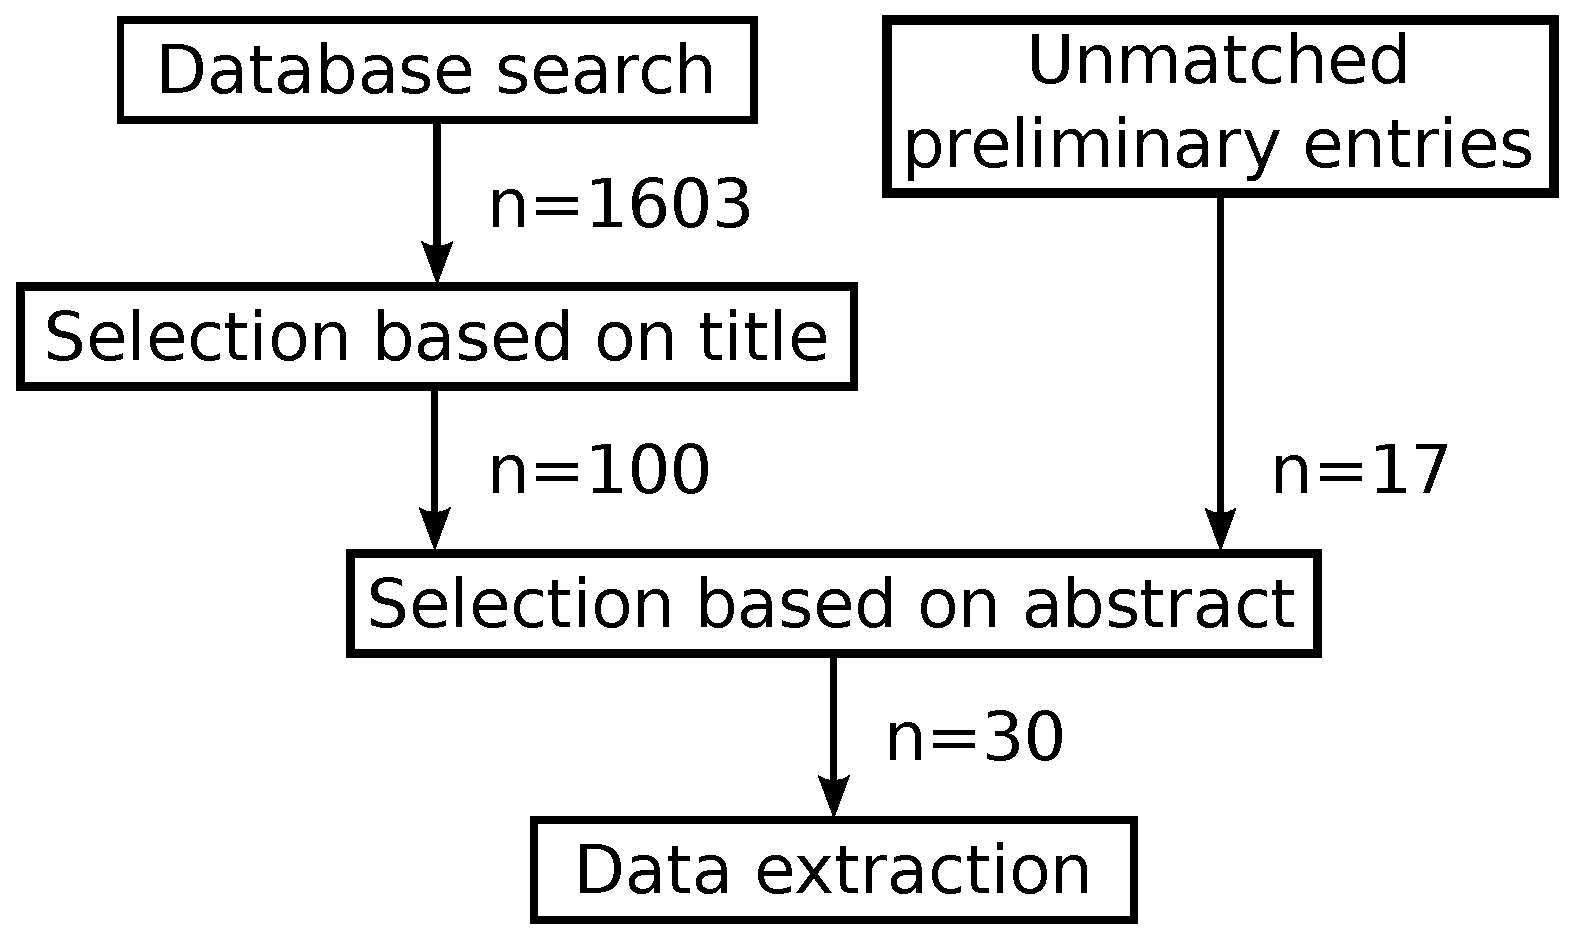
\includegraphics[width=0.5\textwidth]{researchprocess}
    \caption{Process of selecting primary studies}
    \label{fig:selection_process}
  \end{center}
\end{figure}

\subsection{Inclusion criteria}

The 30 primary sources were selected by four criteria: study type, size of
organization, use of agile methods in software development, and viewpoint on
transformation. Firstly, only case studies and experience reports on agile
software development were included in this study. Papers discussing agile
methods or organizational transformation on as a general topic were left out.
Secondly, the size of the organization described in the included primary studies
was to be large enough to show the challenges of large scale agile development
\citegen{Lindvall2004}. Further, only studies discussing agile software development
were included, leaving out for instance studies on agile management. Finally, to
be included each study had to provide a viewpoint on the organizational
transformation.

\subsection{Data extraction}

The content of the resutls was guided by the data extraction form. The form
included some quantitative fields including \textit{start time of
transformation} and \textit{organization size}, but most of the data was
collected in open ended fields. The reason for starting a transformation was
captured in fileds \textit{initial state of organization} and \textit{reasons
for change}. The description of the transformation process was captured in one
field. Recommendations for transformation processes were captured in fields
\textit{reported good practices}, \textit{reported challenges}, and
\textit{lessons learned}. Additional fields that were used but not sufficiently
answered by the primary studies were \textit{satisfaction after transformation},
\textit{effect on onrganization} and \textit{reported measurements before/after
transformation}.

% \begin{table}
%     \begin{tabular}{ p{0.36\textwidth}@{ \hskip 0.2cm } l }
%         \toprule
%         Transformation mentioned in \newline text (Y/N) &
%         Large scale mentioned in text (Y/N) \\
%         Is empirical case study (Y/N) &
%         Is industry experience report (Y/N) \\
%         Has listing of practices (Y/N) &
%         Used research method (Y/N) \\
%         Relevance to this review (1-5) & \\
%         Objective of research (or publication) &
%         Research method \\
%         Author bias &
%         Validity threats \\
%         Organization size &
%         Time of transformation \\
%         Initial state of organization &
%         Why was the change initiated \\
%         How was the change conducted &
%         What is agility? / Which agile paractices are used? \\
%         Findings / lessons learned &
%         Good practices validated or suggested by study \\
%         Reported challenges &
%         Satisfaction after transformation \\
%         Effect on organization &
%         Measurements as results (quantitative or other) \\
%         Other notes &
%         Notable references \\
%         \bottomrule
%     \end{tabular}
%     \caption{The fields of the data extraction form. Fields with a (Y/N) label
%     were answered as yes or no. The field with a (1-5) label was answered by a
%     grade from 1 to 5. All other fields were answered by free form text.}
%     \label{table:dataform}
% \end{table}


%\subsection{Data sources and search strategy}
%
%\subsection{Final selection}
%
%\subsection{Data extraction and synthesis}


% ---------------------------------------------------------------------
\section{Results}
\label{sec:results}

Of the 30 included primary studies 23 were experience reports and 7 were case
studies. From a validity viewpoint it is important to acknowledge that most of
the studies were written by employees in the studied organizations.

All of the included studies had been published within a decade. On average the
studies were published theree years after the transformation was reported to
have begun. Figure \ref{fig:publications} gives a timeline view of the
publications.

\begin{figure}[htb]
  \begin{center}
    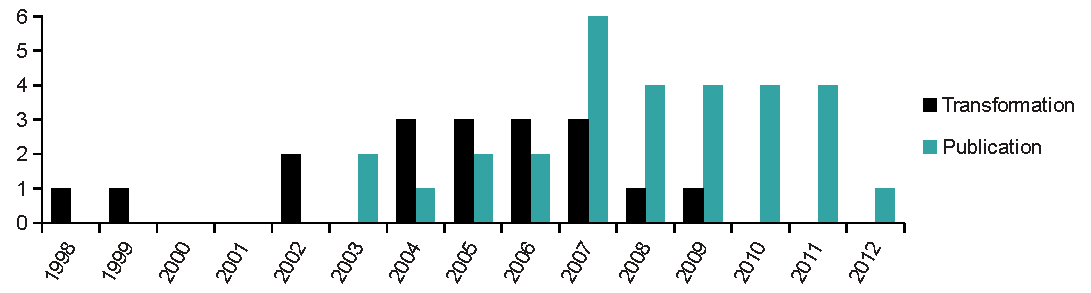
\includegraphics[width=1\textwidth]{publicationschart.pdf}
    \caption{Time of publications and transformations}
    \label{fig:publications}
  \end{center}
\end{figure}


\subsection{Overview of agile methods used}

\begin{table}[h]
    \begin{tabular}{ l@{ \hskip 0.4cm } l }
        \toprule
        Agile method    & Reported in number of studies   \\ \midrule
        Scrum           & 18 \\ 
        XP              & 7 \\
        Lean            & 5 \\
        Tailoring and combining methods & 9  (indirect mentionings not counted) \\
        \bottomrule
    \end{tabular}
    \caption{Reported use of agile methods}
    \label{table:practices}
\end{table}


\subsection{Motivations for transformation}

\begin{table}[h]
    \begin{tabular}{ l@{ \hskip 0.4cm } l }
        \toprule
        Reason                                    & In studies   \\ \midrule
        Need to improve performance               &  \\ 
        Need to eliminate known process problems  &  \\
        Need to improve time to market            &  \\
        \bottomrule
    \end{tabular}
    \caption{Reported resasons for initiating a transformation}
    \label{table:motivations}
\end{table}


\subsection{Typical characteristics of a transformation}

Text only. text. text.


\subsection{Reported challenges}

\begin{table}[h]
    \begin{tabular}{ p{0.36\textwidth} p{0.62\textwidth} }
        \toprule
        Class of challenge  & Examples   \\ \midrule
        
        \raggedright Aligning organization for change  &
             Lack of management support \newline
             Change resistance \newline
             Reverting to old model under pressure \\ 
        
        \raggedright\rule{0pt}{0.4cm}Misunderstanding the agile model  &
             Misinterpretation of roles and responsibilities \newline
             Misunderstanding management role in agile \\
        
        \raggedright\rule{0pt}{0.4cm}Applicability of agile in the organization  &
            Conflicts with business (long term planning) \newline
            Conflicts with other departments (HR) \\
        
        \raggedright\rule{0pt}{0.4cm}Lack of resources  &
            Lack or training, insufficient resources for coaching \\
        \bottomrule
    \end{tabular}
    \caption{Typical challenges encountered in studies}
    \label{table:challenge}
\end{table}


\subsection{Success factors}

\begin{table}[h]
    \begin{tabular}{ p{0.36\textwidth} p{0.62\textwidth} }
        \toprule
        Class of success factors  & Examples   \\ \midrule
        
        \raggedright Organization alignment and leadership  &
             Management support \newline
             Communicating vision for new process \newline
             Demand all organizational units to participate \\ 
        
        \raggedright\rule{0pt}{0.4cm}Coaching and community  &
             Create community to make the new practices stick \\
        
        \raggedright\rule{0pt}{0.4cm}Tailoring and conformity  &
            Invest in tailoring to create the most suitable model \newline
            Conformity clarifies use of the new model \\
        
        \raggedright\rule{0pt}{0.4cm}Investing in change  &
            Training, consulting, physical spaces, tools \\
        \bottomrule
    \end{tabular}
    \caption{Success factors reported in studies}
    \label{table:success}
\end{table}


% ---------------------------------------------------------------------
\section{Conclusions}
\label{sec:conclusions}

-- Research on large scale agile transformations has been published.

-- Papers presenting the effect of agile on specific areas in software
development exist, but the whole has not been studied as much.

\subsection{Limitations}

-- The papers are mostly experience reports with no research method.

-- Some papers were of low quality, but they were included in order to give a
view of the topic that is broader and inclined towards practice.

-- Effect of organizational change is hard (or maybe impossible?) to measure
(kuulemma Marjo ja Kristian tietävät asiasta).

\subsection{Future research}

-- Very little studies on quantitative comparison of before/after transformation
has been done. (how about quantitative?)

-- What thihgs are important to report in an agile transformation case study?

-- Do not focus exclusively on the software perspective, but find parallels from
general research on organizaional transformation and leadership. (Tähän pitäs
vissiin sitte olla joku konkreettinen ehdotus?)


% ---------------------------------------------------------------------
% -------------- BIBLIOGRAPHY -----------------------------------------
% ---------------------------------------------------------------------

\bibliographystyle{plain}
\bibliographystylegen{plain}

\bibliographygen{sources}

\nobibliography{sources_s}

\subsection*{Primary studies}

\begin{supertabular}{ l p{11.3cm} }
    {[}S1{]} & \bibentry{S1} \\ 
    {[}S2{]} & \bibentry{S2} \\ 
    {[}S3{]} & \bibentry{S3} \\ 
    {[}S4{]} & \bibentry{S4} \\ 
    {[}S5{]} & \bibentry{S5} \\ 
    {[}S6{]} & \bibentry{S6} \\ 
    {[}S7{]} & \bibentry{S7} \\ 
    {[}S8{]} & \bibentry{S8} \\ 
    {[}S9{]} & \bibentry{S9} \\ 
    {[}S10{]} & \bibentry{S10} \\ 
    {[}S11{]} & \bibentry{S11} \\ 
    {[}S12{]} & \bibentry{S12} \\ 
    {[}S13{]} & \bibentry{S13} \\ 
    {[}S14{]} & \bibentry{S14} \\ 
    {[}S15{]} & \bibentry{S15} \\ 
    {[}S16{]} & \bibentry{S16} \\ 
    {[}S17{]} & \bibentry{S17} \\ 
    {[}S18{]} & \bibentry{S18} \\ 
    {[}S19{]} & \bibentry{S19} \\ 
    {[}S20{]} & \bibentry{S20} \\ 
    {[}S21{]} & \bibentry{S21} \\ 
    {[}S22{]} & \bibentry{S22} \\ 
    {[}S23{]} & \bibentry{S23} \\ 
    {[}S24{]} & \bibentry{S24} \\ 
    {[}S25{]} & \bibentry{S25} \\ 
    {[}S26{]} & \bibentry{S26} \\ 
    {[}S27{]} & \bibentry{S27} \\ 
    {[}S28{]} & \bibentry{S28} \\ 
    {[}S29{]} & \bibentry{S29} \\ 
    {[}S30{]} & \bibentry{S30} \\ 
\end{supertabular}


\end{document}
